\subsection{C++ particulars}
\label{sec:pf_implementation}

The general construction of the particle filter is straightforward, consisting of Vehicle and Particle objects (as well as the GTFS objects described in \cref{sec:gtfs}). Vehicles are stored within an \verb+std::unordered_map+ using their GTFS \verb+vehicle_id+ as the key.

When a vehicle is first observed, a new Vehicle is created and entered into the map. Then its state is initialised by creating a vector of $\Nparticle$ Particle objects, each of which is assigned a speed between 0 and 30 m/s, and a distance based on the observation:
for GPS observations, map matching is used to determine the approximate location, around which the particle's are scattered;
for trip updates, the particle's are placed at the appropriate stop.
When new data for an existing vehicle is observed, the vehicle's relevant properties are updated (such as position or timestamp). Then the particles are mutated using the transition function from \cref{sec:vehicle_model} and reweighted according to the likelihood function (\cref{sec:pf-likelihood}). If the effective sample size drops below the threshold $\Nthres=\frac{\Np}{4}$, the state is resampled with replacement and particle weights reset to $\frac{1}{\Np}$. See \cref{app:particle-resampling} for details on particle resampling.

Since the vehicles are modelled independently, and they only need to read from the GTFS object (not modify it) the vehicle update step is easily parallelised to use $\tilde M$~cores using the OpenMP library \citep{OMP}. This enables up to a $\tilde M$-fold increase in the speed of this step.

Once the update is complete, the segment index of all particles is obtained, and the \emph{minimum} is used as the vehicle's \emph{current segment}. If this is greater than it was at the end of the previous iteration, the average speed along all intermediate segments is computed by using \verb+std::accumulate+. We also fetch the variance, as so:
\begin{lstlisting}
double avg_speed = std::accumulate(state.begin (), state.end (), 0.0,
  [](double x, Particle& p) {
    return x + p.weight () * p.segment_speed.at (seg_index);
  });
double var_speed = std::accumulate(state.begin (), state.end (), 0.0,
  [&avg_speed](double x, Particle& p) {
    return x + p.weight () *
      pow (p.segment_speed.at (seg_index) - avg_speed, 2.0);
  });
\end{lstlisting}
These observations are then passed to the relevant Segment object which contains a vector of new data (used in chapter 4). The Vehicle object contains a pointer to its Trip, which has a list of Segment objects:
\begin{lstlisting}
trip ()->segments ().at (seg_index)->push_data (avg_speed, var_speed);
\end{lstlisting}

At this point, we have completed modelling the vehicle's state and obtained any available estimates of average road speed.




\begin{figure}
\centering
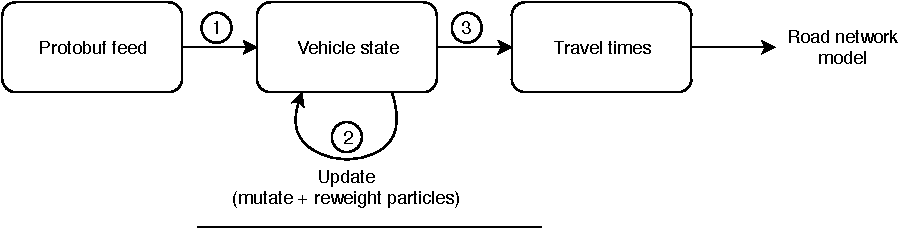
\includegraphics[width=0.8\textwidth,clip,trim={0 1mm 0 0}]{chapters/chapter03/program_overview.pdf}
\caption{Flow diagram of the vehicle model component of the program. Step (1) is the processing of GTFS observations and assignment to vehicles; step (2) is the update (or creation) of vehicle states (via the particle filter); and step (3) is estimation of travel times from the particle trajectories.}
\label{fig:program_flow}
\end{figure}
